% ========================================
% CHAPITRE 1 - PRÉSENTATION DE L'ENTREPRISE D'ACCUEIL
% ========================================

\chapter{Présentation de l'Entreprise d'Accueil}
\label{chap:presentation_entreprise}

\section*{Introduction}

Ce premier chapitre présente l'organisme d'accueil de manière générale et détermine les objectifs et le contexte du stage. Nous commencerons par une présentation succincte du Groupe OCP, avant de nous concentrer sur OCP Maintenance Solutions, la filiale qui nous a accueillis pour ce projet de fin d'études.

Cette présentation permettra de comprendre l'environnement industriel et technologique dans lequel s'inscrit le projet JLHUBSECURITY, ainsi que les enjeux stratégiques qui sous-tendent le développement de solutions digitales innovantes dans le domaine de la sûreté industrielle.

\section{Présentation Générale du Groupe OCP}

\subsection{Introduction au Groupe OCP}

\begin{figure}[h]
\centering

\includegraphics[width=0.4\textwidth]{image/OCP-logo.jpg}
\caption{Logo du Groupe OCP}
\label{fig:logo_ocp}
\end{figure}

L'Office Chérifien des Phosphates (OCP), créé le 7 août 1920 par dahir royal, constitue aujourd'hui l'un des piliers de l'économie marocaine et un acteur incontournable sur la scène internationale. Transformé en société anonyme (OCP SA) en 2008, le groupe s'est imposé comme le leader mondial incontesté dans l'industrie des phosphates et des engrais phosphatés.

\subsubsection{Chiffres Clés du Groupe}

OCP détient une position dominante sur le marché mondial des phosphates avec des indicateurs impressionnants :

\begin{itemize}
\item \textbf{Réserves mondiales} : Accès à plus de 70\% des réserves mondiales de roches phosphatées
\item \textbf{Effectifs} : Près de 23 000 employés
\item \textbf{Part de marché} : 31\% du marché mondial des produits phosphatés
\item \textbf{Production} : Plus de 25 millions de tonnes de phosphate brut par an
\end{itemize}

\subsection{Historique du Groupe OCP}

\subsubsection{Étapes Clés de l'Évolution}

\textbf{1920-1950 : Fondation et premiers développements}
\begin{itemize}
\item \textbf{1920} : Création de l'Office Chérifien des Phosphates par dahir royal le 7 août
\item \textbf{1921} : Début de l'exploitation souterraine sur le gisement des Oulad Abdoun et première exportation de phosphate depuis Casablanca (7 000 tonnes)
\item \textbf{1930} : Ouverture du centre de production de Youssoufia
\end{itemize}

\textbf{1951-1975 : Expansion et modernisation}
\begin{itemize}
\item \textbf{1951} : Démarrage de l'extraction à ciel ouvert à Khouribga et développement des installations de séchage
\item \textbf{1965} : Création de Maroc Chimie et début de la valorisation des phosphates avec l'usine de Safi
\item \textbf{1975} : Formation du Groupe OCP et intégration des industries chimiques aux structures internes
\end{itemize}

\textbf{2008-Présent : Transformation moderne}
\begin{itemize}
\item \textbf{2008} : Transformation historique en société anonyme (OCP SA)
\item \textbf{2014} : Inauguration du pipeline de transport reliant Khouribga à Jorf Lasfar (187 km)
\item \textbf{2024} : Création d'OCP Nutricrops, nouvelle filiale spécialisée
\end{itemize}

\subsection{Structure Organisationnelle}

\begin{figure}[h]
\centering
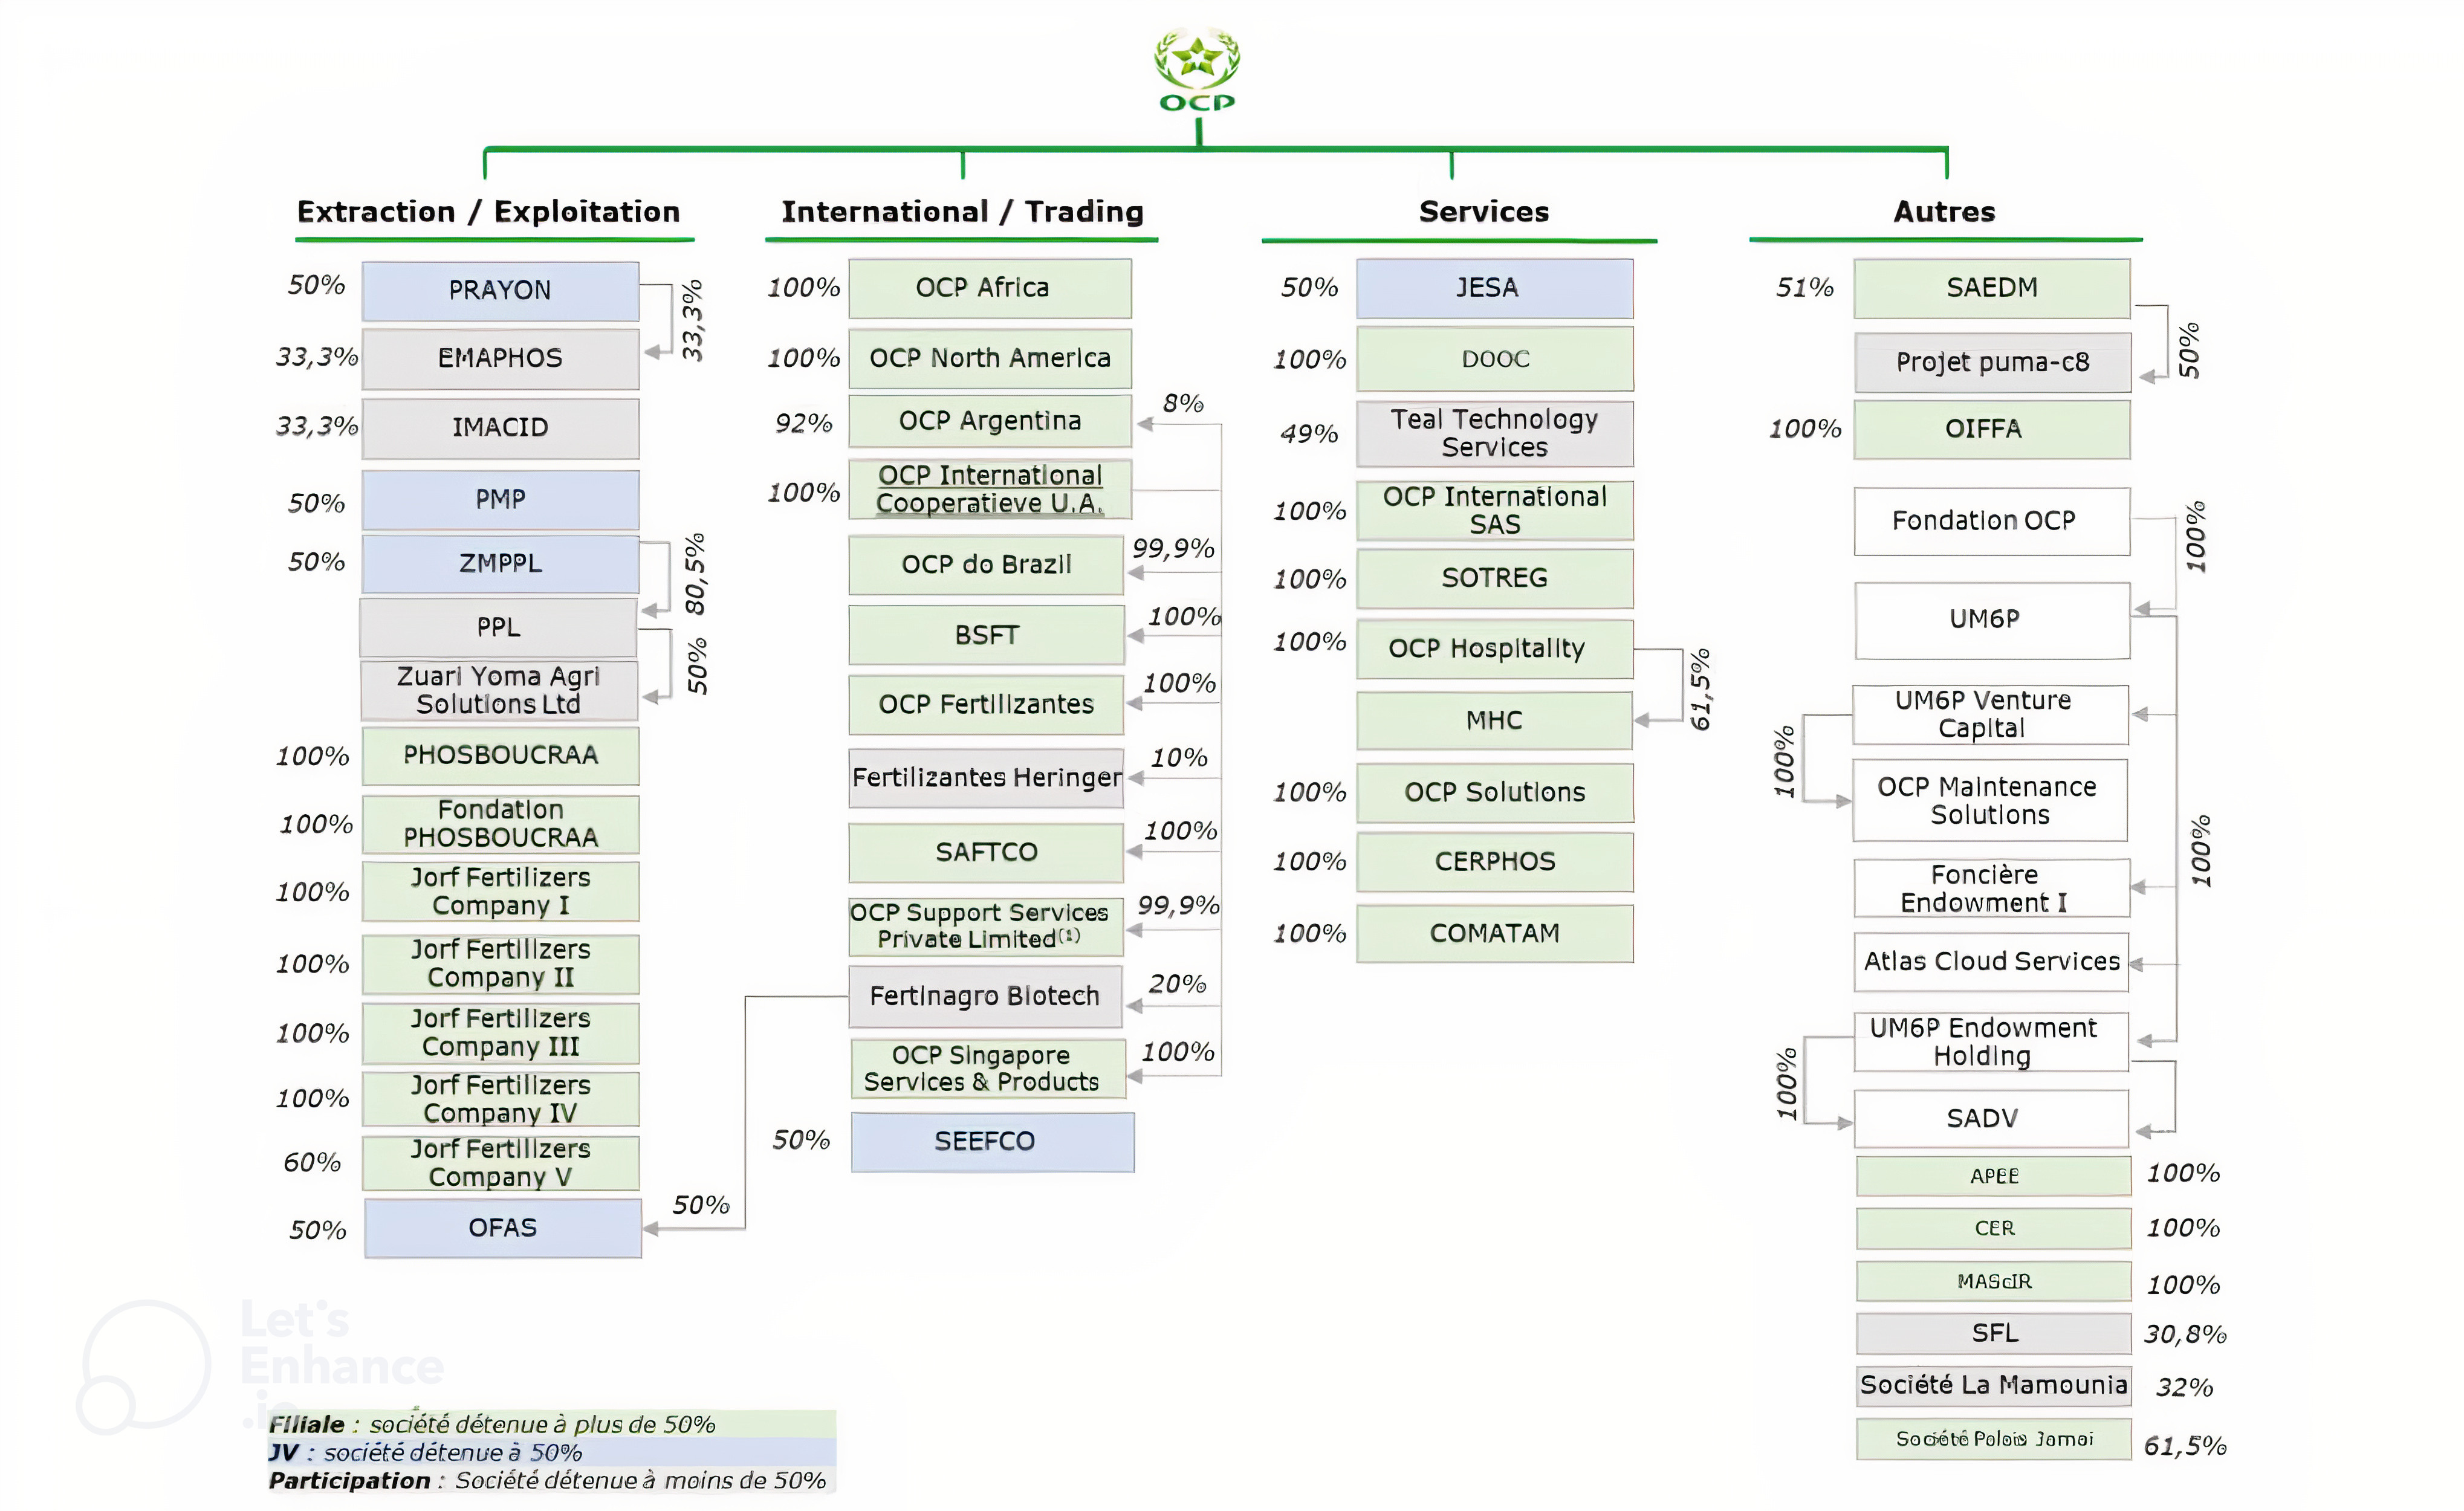
\includegraphics[width=0.8\textwidth]{image/organigramme_ocp.jpg}
\caption{Structure organisationnelle du Groupe OCP avec ses principales filiales}
\label{fig:structure_ocp}
\end{figure}
\newpage

Le Groupe OCP s'appuie sur un écosystème de filiales spécialisées, notamment \textbf{OCP Maintenance Solutions} qui constitue la filiale d'accueil de notre stage et se spécialise dans la digitalisation et la maintenance industrielle 4.0.

\section{OCP Maintenance Solutions : Notre Organisme d'Accueil}

\subsection{Présentation Générale}

\begin{figure}[h]
\centering

\includegraphics[width=0.5\textwidth]{image/ocpms.png}
\caption{Logo d'OCP Maintenance Solutions}
\label{fig:logo_ocp_ms}
\end{figure}

OCP Maintenance Solutions (OCP-MS) représente l'incarnation de la stratégie d'innovation et de digitalisation du Groupe OCP. \textbf{Créée en 2017} comme Business Unit puis transformée en filiale autonome, cette société spécialisée dans la maintenance et la digitalisation industrielle s'est rapidement imposée comme le leader marocain dans les systèmes de surveillance conditionnelle et les services de maintenance prédictive.

\subsection{Mission et Vision Stratégique}

\subsubsection{Mission d'OCP-MS}

La mission d'OCP-MS s'articule autour de trois axes stratégiques fondamentaux :

\textbf{Amélioration de la Productivité :}
\begin{itemize}
\item Optimisation des performances industrielles par l'intégration de technologies avancées
\item Réduction des temps d'arrêt non planifiés de 40\% en moyenne
\item Augmentation de la disponibilité des équipements de 15 à 20\%
\item Optimisation des coûts de maintenance de 25\% grâce à la prédictivité
\end{itemize}

\textbf{Digitalisation et Transformation :}
\begin{itemize}
\item Accompagnement complet de la transformation numérique des entreprises industrielles
\item Développement de solutions IoT et d'intelligence artificielle adaptées au contexte industriel
\item Intégration de plateformes de gestion des données industrielles
\item Mise en place de jumeaux numériques pour les équipements critiques
\end{itemize}

\textbf{Formation et Développement des Compétences :}
\begin{itemize}
\item Développement de l'expertise en maintenance industrielle 4.0
\item Certification des techniciens aux nouvelles technologies
\item Transfert de savoir-faire et de bonnes pratiques
\item Création d'un écosystème de compétences en maintenance prédictive
\end{itemize}

\subsection{Domaines d'Expertise et Solutions Technologiques}

\subsubsection{Maintenance Prédictive et Intelligence Artificielle}



OCP Maintenance Solutions a développé un écosystème technologique complet utilisant les technologies de pointe :

\textbf{Technologies Core :}
\begin{itemize}
\item \textbf{IIOT (Industrial Internet of Things)} : Capteurs intelligents connectés pour collecte de données en temps réel
\item \textbf{Big Data Analytics} : Traitement et analyse de téraoctets de données industrielles
\item \textbf{Machine Learning} : Algorithmes d'apprentissage automatique pour la détection d'anomalies
\item \textbf{Intelligence Artificielle} : Modèles prédictifs avancés pour anticiper les pannes
\end{itemize}

\textbf{Portefeuille de Solutions :}

\textbf{I-SENSE Platform :}
\begin{itemize}
\item Plateforme IoT hautement évolutive et sécurisée
\item Connexion en temps réel de milliers d'équipements
\item Interface web et mobile pour monitoring à distance
\item Tableaux de bord personnalisables par métier
\item Alertes intelligentes et notifications automatiques
\end{itemize}

\textbf{Vibox - Système de Surveillance Conditionnelle :}
\begin{itemize}
\item Protection des machines contre les dommages
\item Surveillance continue de la vibration, température, pression
\item Analyses spectrales avancées
\item Diagnostic automatique des défauts
\item ROI démontré de 300\% en moyenne
\end{itemize}

\textbf{MobiVib - Analyse Vibratoire Mobile :}
\begin{itemize}
\item Kit portable d'acquisition de données
\item Analyse spectrale sur site
\item Mesures haute précision pour équipements rotatifs
\item Rapports automatiques de diagnostic
\item Formation intégrée des opérateurs
\end{itemize}

\subsubsection{Technologies d'Inspection Avancées}

\textbf{Drones d'Inspection Industrielle :}



Acquise en août 2023, cette technologie révolutionnaire permet :

\begin{itemize}
\item \textbf{Inspection thermique} : Détection des points chauds et fuites énergétiques
\item \textbf{Inspection visuelle} : Caméras haute définition pour contrôles visuels
\item \textbf{Zones d'application} : Lignes électriques, panneaux photovoltaïques, pipelines, réservoirs
\item \textbf{Sécurité} : Élimination des risques pour le personnel en environnements dangereux
\item \textbf{Efficacité} : Réduction de 80\% du temps d'inspection
\end{itemize}

\subsubsection{Contrôles Non Destructifs (CND)}

OCP Maintenance Solutions propose une gamme complète de services CND certifiés :

\textbf{Techniques Disponibles :}
\begin{itemize}
\item \textbf{Ultrasons (UT)} : Détection de défauts internes, mesure d'épaisseurs
\item \textbf{Magnétoscopie (MT)} : Contrôle des matériaux ferromagnétiques
\item \textbf{Ressuage (PT)} : Détection de défauts de surface
\item \textbf{Radiographie industrielle (RT)} : Contrôle volumétrique des soudures
\item \textbf{Ultrasons phased array (PAUT)} : Inspection avancée des structures complexes
\item \textbf{Endoscopie industrielle} : Inspection visuelle des espaces confinés
\end{itemize}

\textbf{Secteurs d'Application :}
\begin{itemize}
\item Pétrochimie et raffinerie
\item Centrales électriques
\item Industrie minière
\item Construction métallique
\item Aéronautique
\end{itemize}

\subsection{Formation et Certification - OCP MS Academy}

\subsubsection{Centre d'Excellence en Formation}

\begin{figure}[h]
\centering

\includegraphics[width=0.4\textwidth]{image/ocp_ms_academy.png}
\caption{Centre de formation OCP MS Academy}
\label{fig:ocp_ms_academy}
\end{figure}

OCP MS Academy représente le bras formation de la filiale, avec une approche innovante basée sur le "blended learning" :

\textbf{Programmes de Formation :}
\begin{itemize}
\item \textbf{Analyse vibratoire} : Niveaux I, II, III selon standards ISO 18436
\item \textbf{Maintenance prédictive} : Techniques et technologies émergentes
\item \textbf{IoT industriel} : Déploiement et gestion de capteurs connectés
\item \textbf{Contrôles non destructifs} : Certification selon normes internationales
\item \textbf{Leadership industriel} : Management et soft skills pour l'industrie 4.0
\end{itemize}

\textbf{Méthodologie Pédagogique :}
\begin{itemize}
\item Formation présentielle avec simulateurs industriels
\item E-learning interactif et adaptatif
\item Réalité virtuelle pour situations dangereuses
\item Compagnonnage sur site avec experts
\item Certification continue et évaluation des compétences
\end{itemize}

\subsubsection{Partenariats Internationaux Stratégiques}

\textbf{Mobius Institute (Australie) :}
\begin{itemize}
\item Premier centre certificateur Mobius au Maroc et en Afrique
\item Standards internationaux en analyse vibratoire
\item Plus de 500 techniciens certifiés depuis 2020
\item Reconnaissance mondiale des certifications délivrées
\end{itemize}

\textbf{Nucleom (Canada) :}
\begin{itemize}
\item Partenariat signé en 2021 pour les CND avancés
\item Expertise en inspection de niveau NASA et aerospace
\item Transfert de technologies de pointe
\item Accès aux marchés aéronautique et nucléaire
\end{itemize}

\textbf{Autres Partenaires Technologiques :}
\begin{itemize}
\item \textbf{Wikitude (Autriche)} : Solutions de réalité augmentée
\item \textbf{ifm (Allemagne)} : Capteurs et automatismes industriels
\item \textbf{LARES (Maroc)} : Instruments de métrologie
\item \textbf{BCG Gamma (International)} : Analytics et data science
\end{itemize}

\subsection{Clientèle et Marchés}

\subsubsection{Portefeuille Clients Diversifié}



\textbf{Secteurs d'Intervention :}

\textbf{Cimenterie :}
\begin{itemize}
\item \textbf{Lafarge Holcim} : Contrat de maintenance prédictive sur 5 sites
\item \textbf{Ciments du Maroc} : Surveillance conditionnelle des broyeurs
\item Services : Analyse vibratoire, thermographie, équilibrage
\end{itemize}

\textbf{Sidérurgie et Métallurgie :}
\begin{itemize}
\item \textbf{Universal Industrial Steel} : Partenariat pluriannuel
\item \textbf{Sonasid} : Maintenance prédictive des laminoirs
\item Résultats : Réduction de 60\% des arrêts non planifiés
\end{itemize}

\textbf{Énergie et Utilities :}
\begin{itemize}
\item \textbf{ONEE} : Inspection des centrales thermiques
\item \textbf{Nareva} : Maintenance éoliennes et solaire
\item \textbf{TAQA} : Optimisation des turbines gaz
\end{itemize}

\textbf{Pétrochimie :}
\begin{itemize}
\item \textbf{SAMIR} : Expertise en raffinerie
\item \textbf{Shell Maroc} : Partenariat technologique
\item Spécialités : CND, analyse d'huile, thermographie
\end{itemize}

\textbf{International :}
\begin{itemize}
\item \textbf{Afrique de l'Ouest} : Nigeria, Sénégal, Côte d'Ivoire
\item \textbf{Maghreb} : Tunisie, Algérie (projets pilotes)
\item \textbf{Moyen-Orient} : Émirats Arabes Unis (prospection)
\end{itemize}

\subsubsection{Témoignages Clients}

\begin{quote}
\textit{"La collaboration entre Universal Industrial Steel et OCP Maintenance Solutions dure depuis plusieurs années. Les experts d'OCP-MS nous procurent des analyses pertinentes qui nous ont permis d'améliorer la disponibilité de notre outil industriel et de réaliser des économies considérables."} 

--- Directeur Technique, Universal Industrial Steel
\end{quote}

\begin{quote}
\textit{"Les experts OCP MS sont dévoués et prêts à supporter les équipes opérationnelles pour atteindre une maintenance World Class."} 

--- Responsable Maintenance, Lafarge Holcim
\end{quote}

\subsection{Innovation et Recherche \& Développement}

\subsubsection{Laboratoire d'Innovation}

OCP Maintenance Solutions dispose d'un centre R\&D dédié au développement de solutions "Made in Morocco" :

\textbf{Axes de Recherche :}
\begin{itemize}
\item \textbf{Maintenance 5.0} : Intégration de l'humain dans l'industrie 4.0
\item \textbf{Jumeaux numériques} : Modélisation virtuelle des équipements industriels
\item \textbf{IA explicable} : Algorithmes transparents pour l'aide à la décision
\item \textbf{Edge computing} : Traitement local des données pour réactivité optimale
\end{itemize}

\textbf{Projets de R\&D en Cours :}
\begin{itemize}
\item Développement d'un assistant virtuel pour techniciens de maintenance
\item Plateforme de réalité augmentée pour formation immersive
\item Algorithmes d'optimisation énergétique par IA
\item Solutions de cybersécurité pour l'IoT industriel
\end{itemize}

\subsubsection{Propriété Intellectuelle}

\begin{itemize}
\item \textbf{Brevets déposés} : 5 brevets en cours d'examen
\item \textbf{Solutions propriétaires} : 12 logiciels développés en interne
\item \textbf{Certifications} : ISO 9001, ISO 14001, ISO 45001
\item \textbf{Agréments} : COFREND pour les CND, certification Mobius
\end{itemize}

\subsection{Structure Organisationnelle et Ressources Humaines}

\subsubsection{Organisation et Gouvernance}

\begin{figure}[h]
\centering
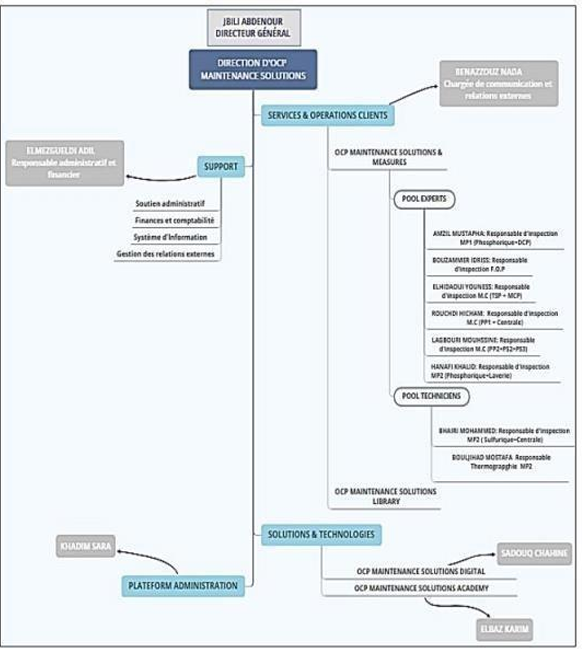
\includegraphics[width=0.8\textwidth]{image/organigramme_ocpms.png}
\caption{Structure organisationnelle d'OCP Maintenance Solutions}
\label{fig:organigramme_ocp_ms}
\end{figure}

\textbf{Direction Générale :}
\begin{itemize}
\item \textbf{Fondateur-Directeur} : Expert maintenance mécanique OCP depuis 2007
\item \textbf{Vision} : Faire d'OCP-MS le leader africain de la maintenance 4.0
\item \textbf{Stratégie} : Croissance organique et acquisitions stratégiques
\end{itemize}

\textbf{Départements Opérationnels :}
\begin{itemize}
\item \textbf{R\&D et Innovation} : 15 ingénieurs et data scientists
\item \textbf{Services Terrain} : 25 techniciens et experts CND
\item \textbf{Formation et Académie} : 8 formateurs certifiés
\item \textbf{Commercial et Marketing} : 6 business developers
\item \textbf{Support et IT} : 6 administrateurs systèmes et support client
\end{itemize}

\subsubsection{Capital Humain}

\textbf{Profil des Collaborateurs :}
\begin{itemize}
\item \textbf{Effectif total} : 60 collaborateurs (objectif 100 en 2025)
\item \textbf{Âge moyen} : 32 ans
\item \textbf{Formation} : 70\% d'ingénieurs, 30\% de techniciens spécialisés
\item \textbf{Genre} : 25\% de femmes (objectif 35\% en 2025)
\item \textbf{Nationalités} : 85\% marocains, 15\% expatriés experts
\end{itemize}

\textbf{Politique RH et Culture d'Entreprise :}
\begin{itemize}
\item \textbf{Formation continue} : 40 heures/an/collaborateur minimum
\item \textbf{Innovation} : 20\% du temps dédié aux projets innovants
\item \textbf{Mobilité} : Rotation inter-sites et missions internationales
\item \textbf{Reconnaissance} : Programme de primes à l'innovation
\end{itemize}

\subsubsection{Philosophie "Mouvement"}

OCP Maintenance Solutions s'inscrit dans la continuité du "Mouvement", initiative stratégique du Groupe OCP pour :

\begin{itemize}
\item \textbf{Libérer le potentiel} : Encourager l'initiative et la créativité
\item \textbf{Intelligence collective} : Favoriser la collaboration inter-métiers
\item \textbf{Agilité} : Adapter rapidement l'organisation aux enjeux
\item \textbf{Entrepreneuriat interne} : Soutenir les projets innovants des collaborateurs
\end{itemize}

\subsection{Stratégie de Développement et Perspectives}

\subsubsection{Plan Stratégique 2024-2027}

\textbf{Objectifs Quantitatifs :}
\begin{itemize}
\item \textbf{Chiffre d'affaires} : Triplement à horizon 2027
\item \textbf{Clients externes} : 50\% du CA (vs 30\% actuellement)
\item \textbf{International} : 25\% du CA depuis les marchés africains
\item \textbf{Innovation} : 15\% du CA investi en R\&D
\end{itemize}

\textbf{Axes de Développement :}
\begin{itemize}
\item \textbf{Expansion géographique} : Bureau au Nigeria et Sénégal
\item \textbf{Diversification sectorielle} : Agroalimentaire, textile, automobile
\item \textbf{Nouveaux services} : Cybersécurité industrielle, efficacité énergétique
\item \textbf{Acquisitions} : Rachat de startups technologiques locales
\end{itemize}

\section{Contexte du Projet JLHUBSECURITY}

\subsection{Positionnement Stratégique dans l'Écosystème OCP}

\subsubsection{Alignement avec la Vision Groupe}



Le système JLHUBSECURITY s'inscrit parfaitement dans la stratégie de digitalisation globale d'OCP Maintenance Solutions et du Groupe OCP. Cette plateforme représente un exemple concret de l'application des technologies Industry 4.0 aux processus de sécurité industrielle, illustrant la capacité d'innovation de la filiale.

\textbf{Cohérence Stratégique :}
\begin{itemize}
\item \textbf{Transformation digitale} : Contribution directe aux objectifs de modernisation
\item \textbf{Sécurité industrielle} : Renforcement des standards de sûreté sur tous les sites
\item \textbf{Innovation technologique} : Démonstration des capacités internes de développement
\item \textbf{Expérience utilisateur} : Amélioration de l'interaction avec les parties prenantes
\end{itemize}

\subsubsection{Enjeux et Défis Sectoriels}

Dans un contexte où la sécurité industrielle devient un enjeu majeur pour les entreprises, particulièrement dans le secteur minier et chimique, OCP Maintenance Solutions développe des solutions innovantes pour répondre aux défis contemporains :

\textbf{Défis Réglementaires :}
\begin{itemize}
\item \textbf{Conformité internationale} : Respect des standards ISO 45001, OHSAS 18001
\item \textbf{Traçabilité renforcée} : Exigences croissantes en matière d'audit et de reporting
\item \textbf{Responsabilité sociétale} : Démonstration de l'engagement sécurité de l'entreprise
\end{itemize}

\textbf{Défis Opérationnels :}
\begin{itemize}
\item \textbf{Digitalisation des processus} : Passage du papier au numérique
\item \textbf{Optimisation des workflows} : Réduction des délais et des erreurs
\item \textbf{Amélioration de l'expérience} : Simplification pour tous les utilisateurs
\item \textbf{Renforcement de la traçabilité} : Contrôle total des mouvements sur site
\end{itemize}

\textbf{Défis Technologiques :}
\begin{itemize}
\item \textbf{Intégration système} : Connexion avec l'écosystème IT existant
\item \textbf{Sécurité des données} : Protection des informations sensibles
\item \textbf{Scalabilité} : Capacité à gérer la croissance des volumes
\item \textbf{Mobilité} : Accès depuis tout type de terminal
\end{itemize}

\subsection{Opportunités et Bénéfices Attendus}

\subsubsection{Bénéfices Opérationnels}

\textbf{Pour OCP Maintenance Solutions :}
\begin{itemize}
\item Démonstration des capacités de développement de solutions métier
\item Référence client interne pour conquérir des marchés externes
\item Développement de compétences en cybersécurité industrielle
\item Création d'une offre produit réplicable sur d'autres sites
\end{itemize}

\textbf{Pour le Groupe OCP :}
\begin{itemize}
\item Modernisation des processus de sûreté sur tous les sites
\item Amélioration de l'image employeur et de l'attractivité
\item Réduction des risques opérationnels et réglementaires
\item Optimisation des coûts de gestion des accès
\end{itemize}

\subsubsection{Impact sur l'Écosystème}

\textbf{Visiteurs et Partenaires :}
\begin{itemize}
\item Expérience d'accès simplifiée et digitalisée
\item Réduction des temps d'attente et des contraintes administratives
\item Meilleure information et accompagnement
\item Image moderne et innovante d'OCP
\end{itemize}

\textbf{Équipes de Sûreté :}
\begin{itemize}
\item Automatisation des tâches administratives répétitives
\item Outils de contrôle et de reporting avancés
\item Amélioration de la traçabilité et de la conformité
\item Réduction de la charge de travail manuelle
\end{itemize}

\section*{Conclusion}

Le Groupe OCP, fort de plus d'un siècle d'expérience et de sa position de leader mondial des phosphates, continue d'innover et de se développer à travers ses filiales spécialisées. Cette capacité d'innovation se manifeste particulièrement à travers OCP Maintenance Solutions, qui illustre parfaitement la transformation de l'entreprise vers l'industrie 4.0.

OCP Maintenance Solutions, par son expertise technologique, sa culture d'innovation et sa vision stratégique, représente l'incarnation parfaite des ambitions de digitalisation du Groupe OCP. La filiale développe des solutions technologiques avancées qui répondent aux enjeux contemporains de l'industrie tout en créant de la valeur pour l'ensemble de l'écosystème.

Le projet JLHUBSECURITY, sur lequel porte ce mémoire, s'inscrit naturellement dans cette dynamique d'innovation et de digitalisation. Il contribue non seulement à l'amélioration des processus de sûreté industrielle au sein d'OCP, mais participe également au renforcement de la position de l'entreprise comme référence en matière de technologies industrielles avancées.

Cette présentation de l'entreprise d'accueil démontre que le projet développé s'appuie sur un environnement d'innovation exceptionnel, des ressources technologiques de premier plan et une vision stratégique claire orientée vers l'excellence opérationnelle et la transformation digitale. Ces éléments constituent un socle solide pour le développement et le déploiement réussi de solutions innovantes comme JLHUBSECURITY.